\documentclass{article}
\usepackage{amsmath, amsthm, amssymb}
\usepackage{listings}
\usepackage{graphicx}
\usepackage{float}
\usepackage{enumerate}
\usepackage{fancyhdr, lastpage,booktabs}
\usepackage{polynom}
\usepackage[left=0.75in, top=1.00in, right=0.75in, bottom=1.00in]{geometry}

\usepackage{graphicx}
\usepackage{tikz}
\usetikzlibrary{backgrounds}
\usepackage{amssymb}

\tikzstyle{cover}=[rectangle,inner sep=1pt,outer sep=0pt]
\tikzstyle{nb}=[fill=red]
\tikzstyle{lv}=[fill=black!80]
\tikzstyle{bd}=[fill=black]

\usepackage{wrapfig}
\usepackage{lmodern}
\usepackage{blindtext}

\usepackage{float}
\restylefloat{figure}

\pagestyle{fancy}
\setlength{\headheight}{24pt}

\makeatletter
\renewcommand*\env@matrix[1][*\c@MaxMatrixCols c]{%
  \hskip -\arraycolsep
  \let\@ifnextchar\new@ifnextchar
  \array{#1}}
\makeatother

\newcommand {\otoprule }{\midrule [\heavyrulewidth]}

\begin{document}
  
    \rhead{Fred Eisele\\MA 274: 2011 May 3}
    \cfoot{\thepage\ of \pageref{LastPage}}

\setlength{\parskip}{5mm}

 
\section*{1(a)}

\framebox[\linewidth][l]{
\begin{minipage}{0.9\linewidth}
Consider one of the available John Conway's Game of Life
implementations.
Discover patterns that lead to each of the four different classes of behaviors.
Include screen captures of the evolution of the different patterns in time,
and generate an explanation of why the different behaviors emerge and why
you classified it as such.
\end{minipage}
 }
 
 \begin{figure}[H]
   \centering
 
 \begin{tikzpicture}[x=0.1\textwidth, y=0.1\textwidth]

\fill[lv] (1,0) rectangle (2,1);
\fill[lv] (0,1) rectangle (1,2);
\fill[lv] (0,2) rectangle (1,3);
\fill[lv] (1,2) rectangle (2,3);
\fill[lv] (3,1) rectangle (4,2);
\fill[lv] (2,3) rectangle (3,4);

\draw[-] [bd] (-1,0)--(5,0);
\draw[-] [bd] (-1,1)--(5,1);
\draw[-] [bd] (-1,2)--(5,2);
\draw[-] [bd] (-1,3)--(5,3);
\draw[-] [bd] (-1,4)--(5,4);
\draw[-] [bd] (0,-1)--(0,5);
\draw[-] [bd] (1,-1)--(1,5);
\draw[-] [bd] (2,-1)--(2,5);
\draw[-] [bd] (3,-1)--(3,5);
\draw[-] [bd] (4,-1)--(4,5);

\fill[nb] (.5,3.5) circle (0.2);
\fill[nb] (.5,2.5) circle (0.2);
\fill[nb] (.5,1.5) circle (0.2);
\fill[nb] (1.5,1.5) circle (0.2);
\fill[nb] (2.5,1.5) circle (0.2);
\fill[nb] (2.5,2.5) circle (0.2);
\fill[nb] (2.5,3.5) circle (0.2);
\fill[nb] (1.5,3.5) circle (0.2);

\end{tikzpicture}
 \caption{Friend v. Gift Preference Board}\label{fig:board}
\end{figure}
 
 The mapping restriction from friends to gifts can be represented as a board
 where marked squares indicate the friends dislike for a particular gift.
 For that board finding the number of giving exactly $ k = 3 $ gifts
 $ e_m $ for  where all of the gifts are acceptable $ m=0 $.
 There are $ n = 5 $ friends and $ m = 7 $ gifts.
 
 This can be done using either the rook polynomial $ R(x,B) $ directly
 or by first finding the rook polynomial for the complementary board 
 $ R(x,\overline{B}) $.
 
 \begin{figure}[H]
   \centering
   \begin{tikzpicture}
     \path (-1,4.5) node (va) {$A$};
     \path (-1,3.5) node (va) {$B$};
     \path (-1,2.5) node (vb) {$C$};
     \path (-1,1.5) node (vb) {$D$};
     \path (-1,0.5) node (vb) {$E$};
     
     \path (0.5,5.5) node (vb) {$1$};
     \path (1.5,5.5) node (vb) {$2$};
     \path (2.5,5.5) node (vb) {$3$};
     \path (3.5,5.5) node (vb) {$4$};
     \path (4.5,5.5) node (vb) {$5$};
     \path (5.5,5.5) node (vb) {$6$};
     \path (6.5,5.5) node (vb) {$7$};
     
     \fill[gray] (0,5) rectangle (1,4) ;
     \fill[gray] (1,2) rectangle (2,3) ;
     \fill[gray] (2,0) rectangle (3,1) ;
     \fill[gray] (3,3) rectangle (4,4) ;
     \fill[gray] (3,1) rectangle (5,2) ;
     \fill[gray] (5,3) rectangle (6,4) ;
     \fill[gray] (6,0) rectangle (7,1) ;
     
     \draw (0,0) grid (7,5);
     
   \end{tikzpicture}
   \caption{Friend v. Gift Preference Board}\label{fig:board}
 \end{figure}
 
 Find the complement rook polynomial of Figure \ref{fig:board}
 
 \begin{align}
R(x,\overline{B}) &= \left( 
\begin{tikzpicture}[scale=0.5]
     \draw (0,0) grid (1,1);
   \end{tikzpicture} \right)^2
   \cdot \left( 
   \begin{tikzpicture}[scale=0.5]
     \draw (0,0) grid (2,1);
   \end{tikzpicture} 
    \right) \cdot \left( 
   \begin{tikzpicture}[scale=0.5]
     \draw (1,0) grid (3,1);
         \draw (0,1) grid (2,2);
      \path (1.5,1.5) node (s1) {$s$};
   \end{tikzpicture} \right)  \label{eqn:boards} \\
  &= \left( 
  \begin{tikzpicture}[scale=0.5]
     \draw (0,0) grid (1,1);
   \end{tikzpicture} \right)^2
   \cdot \left( 
   \begin{tikzpicture}[scale=0.5]
     \draw (0,0) grid (2,1);
   \end{tikzpicture} 
    \right) \cdot \left[ \left(
   \begin{tikzpicture}[scale=0.5]
     \draw (0,1) grid (1,2);
         \draw (1,0) grid (3,1);
         \path (1.5,1.5) node (s1) {$s$};
   \end{tikzpicture} \right) + 
   x  \left(
   \begin{tikzpicture}[scale=0.5]
     \draw (2,0) grid (3,1);
     \path (1.5,1.5) node (s1) {$s$};
   \end{tikzpicture} \right) \right]  \\
   &= (1+x)^2 (1+2x) [(1+x) (1+2x) + x(1+x)] \\
   &= (1+2x+x^2) (1+2x) [(1+3x+2x^2) + (x+x^2)] \\
   &= (1+2x+x^2) (1+2x) (1+4x+3x^2)  \\
   &= (1 + 4x + 5 x^2 + 2 x^3) (1+4x+3x^2)  \\
   &= 1 + (4+4)x + (5+16+3)x^2 + (2+20+3)x^3 +(8+15)x^4+(6)x^5  \\
R(x,\overline{B})  &= 1+8x + 24 x^2 + 34 x^3 + 23 x^4 + 6 x^5
\end{align}
 
 We have the formula for the coefficients of rook polynomials 
 $ R(x,B) = \sum_{j=0}^{\infty} r_j(B) x^j $.
 We also have an identity 
 $ s_j = r_j(\overline{B} \dbinom{m-j}{k-j} \dbinom{n-j}{k-j} (k-j)! $.
 
From which the $ s_j $ terms can be calculated.
\begin{equation}
\begin{array}{rccc}
 s_0 &= 1 \cdot \binom{5}{3} \cdot \binom{7}{3} 3! &=  1 \cdot 10 \cdot 35 \cdot 6 &= 2100 \\
 s_1 &= 8 \cdot \binom{4}{2} \cdot \binom{6}{2} 2! &=  8 \cdot 6 \cdot 15 \cdot 2 &= 1440 \\
 s_2 &= 24 \cdot \binom{3}{1} \cdot \binom{5}{1} 1! &= 24 \cdot 3 \cdot 5 \cdot 1&= 360 \\
 s_3 &= 34 \cdot \binom{2}{0} \cdot \binom{4}{0} 0! &=  34 \cdot 1 \cdot 1 \cdot 1 &= 34 \\
 s_j &= r|j \cdot 0\cdot 0 ? &=  0 &= \text{when } j \ge 4
\end{array}
\end{equation}

\begin{align}
 e_0 &= s_0 - s_1 + s_2 - s_3 + s4 + \cdots \\
  &= 2100 - 1440 + 360 - 34 + 0 \\
e_0 &= 986
\end{align}
There are 986 ways to give exactly three of the seven gifts to the five friends 
without giving more than one gift to any friend and without giving any gift
to someone who does not want it.
\qed

\end{document}

